\documentclass[%
	pdftex,
	oneside,        % One-sided print
	11pt,           % Font size
	parskip=half,   % The half of a line margin after line feeds
	headsepline,    % Line after header
	footsepline,    % Line after footer
	abstracton,     % Abstract headings
	USenglish,      % Written in English
	a4paper,        % Written on Din A4 paper
]{report}


\title{Knowledge based systems\\ Analysing the eligibility of a person for higher education using a Bayesian network}
\author{Lisa Mischer \& Frank Steiler\\ Interactive and knowledge based systems (T2INF4307)\\ DHBW Stuttgart\\ Contact: it12147@lehre.dhbw-stuttgart.de}
        
\usepackage[english]{babel}
\usepackage[english=british]{csquotes}
\usepackage[style=alphabetic,backend=biber,natbib=true]{biblatex}
\addbibresource{Documentation.bib}
\usepackage{graphicx}
\usepackage{setspace}
\usepackage{hyperref}
\usepackage{varioref}
\usepackage{chngcntr}
\usepackage{subcaption}
\usepackage[export]{adjustbox}[2011/08/13]
\usepackage{fancyhdr}
\usepackage[toc,page]{appendix}
\usepackage{pdfpages}
\usepackage{tabularx}
\usepackage{longtable}
\usepackage{float}
\usepackage{pifont}
\usepackage{rotating}
\usepackage{pdflscape}

\usepackage{color}
\definecolor{ListingBackground}{rgb}{0.92,0.92,0.92}

\usepackage{listings}
\lstset{
    basicstyle=\normalfont\ttfamily,
    language=java,
    extendedchars=true,
    backgroundcolor=\color{ListingBackground},
    frame=single,
    numbers=left,
    tabsize=8,
    numberstyle=\scriptsize,
    stepnumber=1,
    numbersep=8pt,
    keepspaces=true, 
    breaklines=true,
    showstringspaces=false
}

\hypersetup{
	colorlinks=true,
    citecolor=black,
    filecolor=black,
    linkcolor=black,
    urlcolor=black,
	pdftitle=Analysing the eligibility of a person for higher education using a Bayesian network,
	pdfauthor={Lisa Mischer \& Frank Steiler}, 
	pdfcreator={Lisa Mischer \& Frank Steiler},
	pdfproducer={Lisa Mischer \& Frank Steiler},
	pdfdisplaydoctitle=true
}

\restylefloat{table}

\onehalfspacing


\pagestyle{fancy}
\lhead{}
\renewcommand{\headrulewidth}{0pt}
\setlength{\headheight}{14pt}

\newcommand{\nocontentsline}[3]{}
\newcommand{\tocless}[2]{\bgroup\let\addcontentsline=\nocontentsline#1{#2}\egroup}

\begin{document}

\counterwithout{figure}{chapter}
\counterwithout{table}{chapter}
\counterwithout{lstlisting}{chapter}

\newcounter{magicrownumbers}[table]

\maketitle

\newpage
\thispagestyle{empty}
\mbox{}
\setcounter{page}{0}

\tableofcontents

\chapter{Introduction}
Within knowledge based systems, logic is a commonly used way to represent connections between data and expressions. Unfortunately logic can not handle uncertainty or imprecise data. Bayesian Networks have been developed to tackle this problem, by representing knowledge as a set of variables and their dependencies within a directed acyclic graph. \cite{Reichardt:2014aa}

A probabilistic network is using conditional probabilities between the nodes of the graph and inferences to calculate the probability of symptoms and/or causes. There are three types of inferences that are occurring in the network and enable the functionality of the graph: diagnostic, causal and inter-causal inference.

A Bayesian Network is defined by a set of edges (nodes) connected through vertices within a graph: $D=(V,E)$. Every node has finite set of mutually exclusive states. On top of that the network is quantifying the dependencies within a separated conditional probability table (CPT) for each node. \cite{Vomlel:2005aa}

Concluding to create and then use a Bayesian Network, a user has to create the correct graph first and then determine all values for the CPT. A correct network can either be created by an expert, by using data mining techniques to find connections between entities and machine learning to specify the CPT values. 

By adding observations for a specific case to the network, it is updating beliefs about other variables. Furthermore the probability of a certain event or state can be predicted by observing other events or states. Therefore it can support decision making and has numerous applications, like the diagnosis of diseases, automatic troubleshooting or education testing. \cite{Vomlel:2005aa}

\chapter{Preparation of data}
As part of our exercise we received a set of data that was supposed to help us derive the structure of the network. To be able to use the stated cases we first had to analyse and harmonise the provided data. 

These preparation included the transformation of continuous variables into discrete ones, to enable their usage within the network. The variables we had to adjust were all provided grades, the test results of the online tests and study ability test, as well as the parental income. 

Furthermore we chose a general syntax for the naming of values, to have standardised identifiers and consistent ranges. E.g. we defined a not available value as "NA", where the source used different words in different entities, like "keine", "n.a." and many more. We did not need to do this necessarily, but it simplified the work with the network.

A detailed description about the conversation of these values can be found within the documentation of the implementation in chapter \vref{chapter:WhatToStudy}, more specific in section \vref{sec:CaseFile}.

These preparations were necessary to train the Bayesian network, as well as to analyse a certain case. Only cases which are prepared in the same way can be evaluated with our result network, but the implementation is able to read a cleaned

\chapter{Structure of the network}
To find the best structure of the network, we took a look at the provided information, trying to find connections between columns of the data set. 

Therefore we plotted the data within a parallel coordinate system, shown in appendix \vref{app:Parallel}. We used this representation to derive connections by reducing the data on a single axis to a smaller range and hoping to observe a similar behaviour on another axis. By revealing such a influence we concluded a direct connection between the entities.

On top of that we thought about logical connections, e.g. the mathematics', German's and physic's grade had to influence the qualification average. Furthermore, we took it for granted that the mathematics grade influences the results of the math online test, as well as the German grade influences the results of the German online test. Moreover the mathematics results influence the physics grade, since a basic understanding of mathematics is essential for physics. 

To determine whether or not our Bayesian network is suited to predict the final grade of a specific student, we tested it using the provided data set. This test tried to predict the final grade of a person, using all available information from the data excluding the actual course and the actual final grade. By comparing the predicted and the actual result, we received an error rate for our network. We used this error rate to compare different versions of the network.

The generation of the final network was an iterative process, changing the arcs, CPTs and/or entities within each step. After changing the structure, we determined the new error rate and compared it to the previous one. By using this process we were able to improve the overall performance of the network. In the end, all our considerations at the beginning proved as wrong, since there is no indirect influence on a variable, only direct.

We were able to achieved an error rate of 11\%, predicting the course taken, and 4\%, predicting the final grade of a student. Appendix \vref{app:Network} is showing our final Bayesian network. The implementation documented in chapter \vref{chapter:WhatToStudy} is using a slightly different Network, since the optimal one is too big, resulting in a out of memory error of the Java virtual machine. In the adjusted net the gender of a person is no longer considered, to reduce its size. Nevertheless, the error rate only rises slightly to 14\%, respectively 6\%. This network is then used to recommend for or against studying a specific course. 

The tool we used to specify our Bayesian network is called Netica, unfortunately we only had access to a limited version of this program. Concluding, it was necessary to limit our data set to 15 entities. Therefore we had to leave out at least one piece of information and take a slightly more imprecise result into account. We chose to ignore the information about the state, even though it improved the error rate significantly, when taking only 5 of 16 states into account. Unfortunately it is necessary to accept all 16 available states, since all of them could be chosen. This resulted in an entity with 16 different parameter values, which were too much to handle for Netica. Since it was not reasonable to allow only 5 parameter values, we decided to leave this entity out of consideration. Furthermore we left out the income of the parents and the nationality, since these did not provide any gain in information to the network.

\chapter{Learning conditional probability tables}
\label{chapter:Learning}
After creating a draft of the network layout, containing all plausible node connections, we had to quantify the dependencies between nodes within the conditional probability tables (CPT). Since we were not able to consult an expert about this problem we chose to use machine learning algorithms to generate the tables.

Fortunately the tool we used to specify the network offered a set of machine learning algorithms to generate the CPTs from a data set. These include a \enquote{counting algorithm}, an \enquote{expectation-maximization (EM) algorithm} and a \enquote{gradient descent algorithm}. According to the documentation of the tool the \enquote{counting algorithm} is the simplest and fastest. This algorithm is especially well performing when having no uncertainty or missing data. Concluding if the data set has missing values, the user should either choose the \enquote{EM-algorithm} or the \enquote{gradient descent algorithm}. The performance of either is highly depending on the data set and network structure. Therefore the selection of one algorithm over the other needs to be done by directly comparing their performance. \cite[p. 47]{Corp.:2010aa} 

After comparing the performance of each algorithm using our set of data, we chose to use the \enquote{expectation-maximization (EM) algorithm}, since it fitted our needs best. \enquote{Briefly, Expectation Maximization learning repeatedly takes a Bayes net and uses it to find a better one by doing an expectation step followed by a maximization step. In the expectation step, it uses regular Bayes net inference with the existing Bayes net to compute the expected value of all the missing data, and then the maximization step finds the maximum likelihood Bayes net given the now extended data.} \cite[p. 48]{Corp.:2010aa}

After applying the algorithm with several hundert iterations using the provided data set we could create a network that reliably predicted the final grade and therefore could give a recommendation based on all provided values. As mentioned earlier the error rate at predicting the final grade correctly is 4\%. Testing the quality of the network based on the correct recommendation of studying the selected course and using the worse network mentioned in chapter \vref{chapter:Learning}, achieves an error rate of 2\%, where no error is false positive (Recommending the course even if the student is probably not going to succeed). This testing is done within the application and its precise documentation can be found in section \vref{sec:Test}.

\chapter{Implementation - WhatToStudy}
\label{chapter:WhatToStudy}
\section{General usage}

\section{Operation modes}
\subsection{Interactive mode}
\subsection{Evaluation mode}
\subsection{Draw mode}
\subsection{Learning mode}
\label{sec:Test}
\subsection{Testing mode}
\subsection{Help mode}
\subsection{Version printing mode}

\section{Case file handling}
\label{sec:CaseFile}
%Include source code from file using:
%\lstinputlisting[caption=Expected output for the program (implemented using the Bridge design pattern)]{./Source/de/steilerdev/swe/Bridge/output}

\lstlistoflistings
\printbibliography

\begin{appendices}

%Include pdf for appendix using:
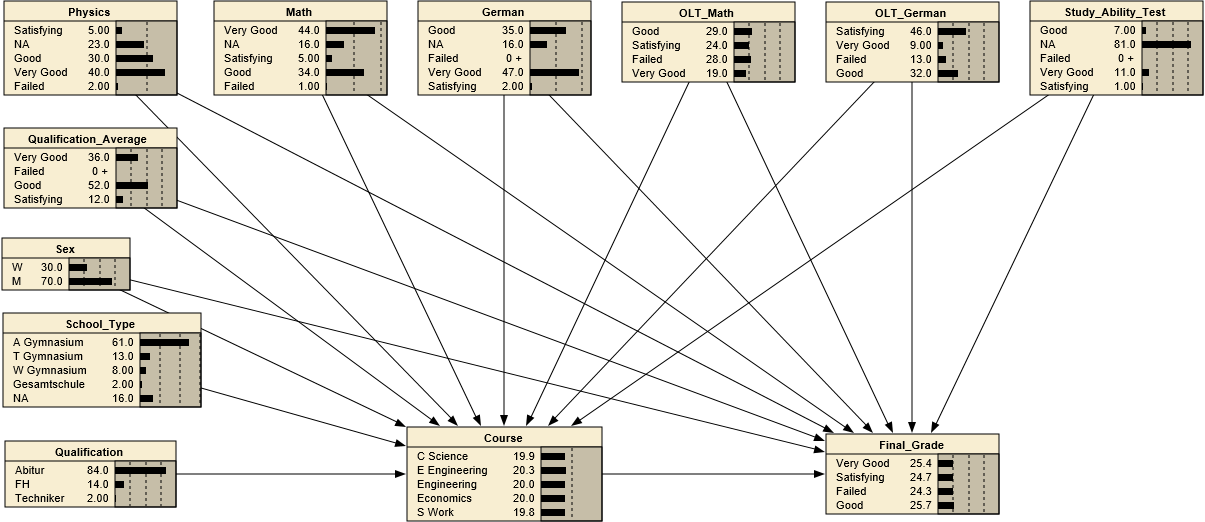
\includepdf[landscape=true,pages=-,addtotoc={1,chapter,0,Bayesian Network,app:Network}]{./assets/StudyNet_Optimal.png}
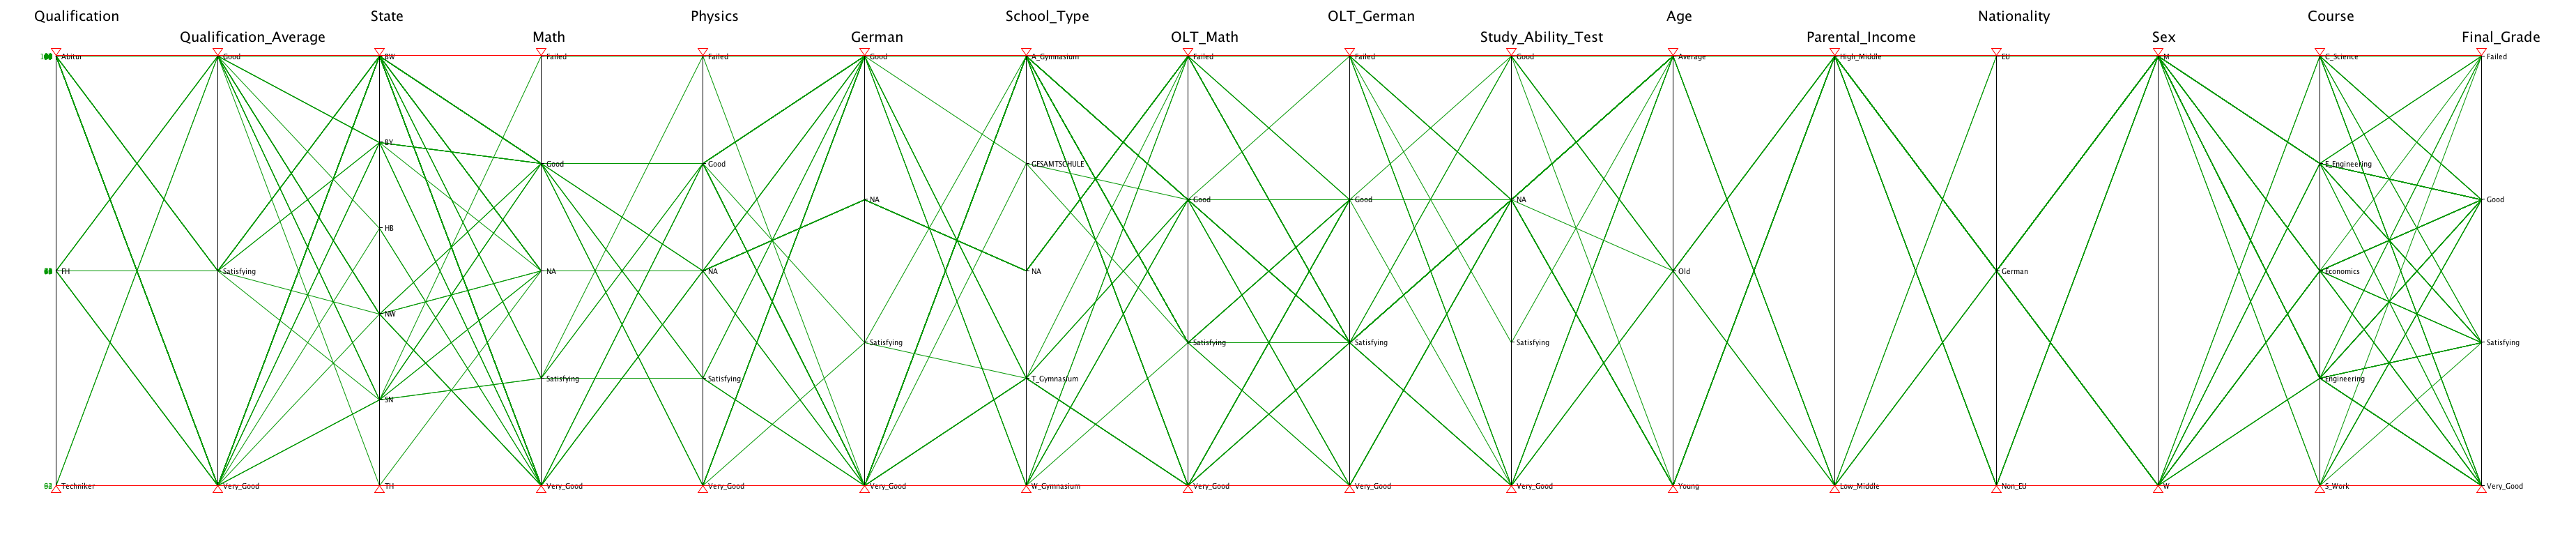
\includepdf[landscape=true,pages=-,addtotoc={1,chapter,0,Data set represented by parallel coordinates,app:Parallel}]{./assets/Parallel.png}

\end{appendices}

\end{document}